% This is samplepaper.tex, a sample chapter demonstrating the
% LLNCS macro package for Springer Computer Science proceedings;
% Version 2.20 of 2017/10/04
%
\documentclass[runningheads]{llncs}
%
\usepackage{graphicx}
% Used for displaying a sample figure. If possible, figure files should
% be included in EPS format.
%
% If you use the hyperref package, please uncomment the following line
% to display URLs in blue roman font according to Springer's eBook style:
% \renewcommand\UrlFont{\color{blue}\rmfamily}
\usepackage{fullpage}
\usepackage{float}

\begin{document}
%
\pagenumbering{gobble}
\title{Reconhecimento de padrões (Perceptron)}
%
%\titlerunning{Abbreviated paper title}
% If the paper title is too long for the running head, you can set
% an abbreviated paper title here
%
\pagestyle{plain}
\author{Autores: Gabrielle Cibyl da Hora; Marco Vallim \\ 
Diciplina: Computação Natural \\
Professor: Leandro Nunes de Castro} 
%
%\authorrunning{F. Author et al.}
% First names are abbreviated in the running head.
% If there are more than two authors, 'et al.' is used.
%
\institute{PPGEEC - Programa de pós-graduação em Engenharia Elétrica e Computação. 
Universidade Presbiteriana Mackenzie.}
%
\maketitle              % typeset the header of the contribution
%
\begin{abstract}
O relatório de pesquisa propõe implementação, execução e análise. Utilizando algoritmo Perceptron e parâmetros pré-definidos identificamos o comportamento de classificação de redes neurais.

\keywords{Redes Neurais  \and Perceptron  \and Computação Natural }
\end{abstract}
%
%
%\
\section{Introdução}

Redes neurais artificiais têm recebido muita atenção devido à sua capacidade de processamento de imagem, reconhecimento de fala, linguagem natural, entre outras aplicações. Algumas das principais tarefas realizadas por elas são classificações, predições e identificação de padrões. \cite{Cao17} 

Uma rede neural artificial é um sistema computacional que busca simular o funcionamento do cérebro humano para processar dados. Por meio desta metáfora com o sistema nervoso humano, é possível compreender a estrutura e o funcionamento dessas redes que são compostas por neurônios e sinapses. \cite{Cao17}

Podemos definir os neurônios como unidades de processamento que realizam uma soma ponderada de seus sinais de entrada e são distribuídos em camadas de entrada, saída e camadas ocultas. Estas camadas são interligadas pelas sinapses que representam as conexões neurais, responsáveis pelo envio dos sinais. \cite{Cao17} \cite{M} 

As redes neurais buscam otimizar os pesos dos parâmetros que serão calculados pelos neurônios. Elas aprendem por meio de um processo de treinamento, no qual o modelo recebe um conjunto de dados de entrada a serem processadas, buscando a identificação de padrões e a saída esperada para cada conjunto de observações, norteando o processo de aprendizagem. \cite{M}

Entre os diversos tipos diferentes de redes neurais, destancam-se os \textit{Multilayer perceptron (MLP)} que possuem três ou mais camadas e utilizam uma função de ativação não linear e cada neurônio. Nas MLPs, uma camada se conecta a cada neurônio na camada seguinte, tornando a rede totalmente conectada.  \cite{M} 
O Perceptron Multicamadas (\textit{Multi-Layer perceptron}) é um classificador de rede neural de classificação simples e linear, ou seja, é um algoritmo que separa linearmente elementos de grupos que tenham características diferentes, e com base nessa separação prever a qual grupo pertencerá elementos não classificados previamente.




\section{Algoritmo}

\begin{figure}
\begin{center}
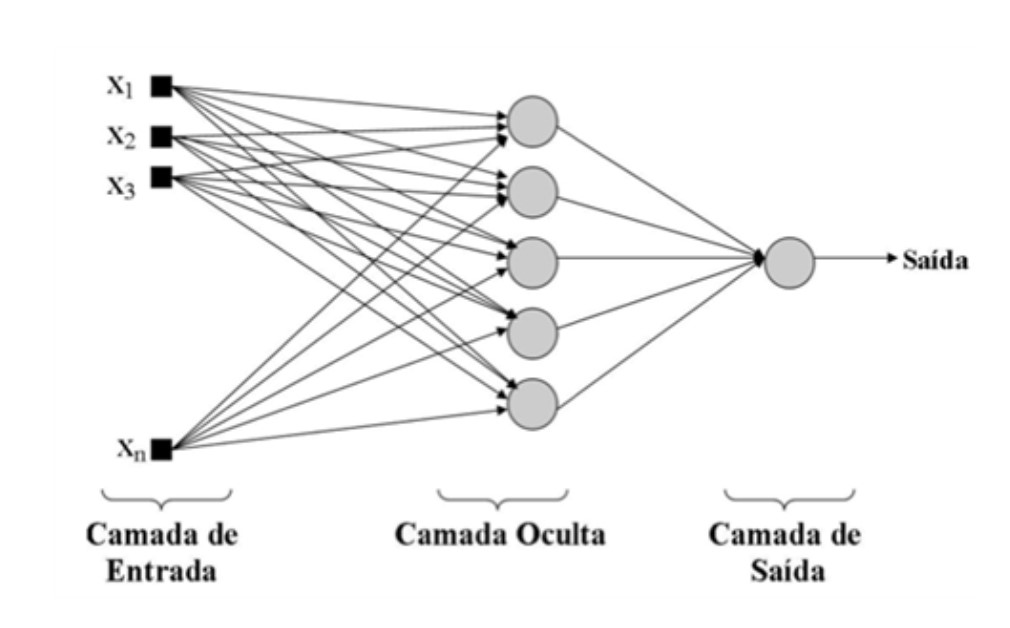
\includegraphics[scale=0.30]{fluxograma.jpg}
\end{center}
\caption{A figura representa o algoritmo genético executado} \label{fig1}
\end{figure}

Fluxo do algoritmo (exemplificado na Fig 1.):
\begin{enumerate}
	\item Iniciar com a entrada parametrizada pelo arquivo de entrada pré definido pela atividade.
	\item Na fase de ativação, calcula-se os valores dos neurônios da camada oculta e dos neurônios da camada de saída
	\item Aplica-se a mutação 1 (inverte o valor do elemento com o próximo a direita), ou mutação 2 (seleciona dois cromossomos aleatórios e troca).
	\item Durante a fase de treinamento verifica os erros dos neurônios das camadas de saída e oculta, correção dos pesos e atualização.
	\item Repetir a partir do item 2 até que melhore o critério de erro
\end{enumerate}

\section{Metodologia}

\subsection{Perceptron}

\subsection{Hiperparametrização do algoritmo}


\subsection{Forma/medida de avaliação de desempenho}

\subsection{Experimentos}


O projeto consiste em ter um gene fixo e realizar diferentes experimentos com diversas combinações de parâmetros para identificação de desempenho, conforme especificado na sessão 3.2. 


\section{Conclusão}

%
% ---- Bibliography ----
%
% BibTeX users should specify bibliography style 'splncs04'.
% References will then be sorted and formatted in the correct style.
%
% \bibliographystyle{splncs04}
% \bibliography{mybibliography}
%

\begin{thebibliography}{8}
\bibitem{Cao17}
Cao, Weipeng; Wang, Xi-Zhao; Ming, Zhong; Gao, Jinzhu.: A Review on Neural Networks with Random Weights. Neurocomputing. 275. (2017) 10.1016/j.neucom.2017.08.040. 

\bibitem{M}
Mohammadi, Mohammad Reza; Sadrossadat, Sayed Alireza; Mortazavi, Mir Gholamreza; Nouri, Behzad.: A brief review over neural network modeling techniques. IEEE International Conference on Power, Control, Signals and Instrumentation Engineering (ICPCSI). 54--57. (2017)


\end{thebibliography}

\end{document}
